\documentclass{article}
\usepackage{fancyhdr}
\usepackage{ctex}
\usepackage[a4paper, body={18cm,22cm}]{geometry}
\usepackage{amsmath,amssymb,amstext,wasysym,enumerate,graphicx}
\usepackage{float,abstract,booktabs,indentfirst,amsmath}
\usepackage{multirow}
\usepackage{enumitem}
\usepackage{xcolor}
\usepackage{tabularx}
\usepackage[most]{tcolorbox}
\usepackage{accsupp}
\usepackage[bottom]{footmisc}
\usepackage{subcaption}
\usepackage{logicproof}
% \usepackage[backend=biber,style=numeric]{biblatex}
\usepackage[xetex]{hyperref}
\usepackage{fontspec}
\usepackage{listingsutf8}
\usepackage{xcolor}
\usetikzlibrary{arrows.meta}
\newcommand\emptyaccsupp[1]{\BeginAccSupp{ActualText={}}#1\EndAccSupp{}}
\setlength{\parindent}{2em}
\setmonofont{Consolas}
\setCJKmonofont{黑体}
% \setmainfont{Times New Roman}
\hypersetup{CJKbookmarks=true,colorlinks=true,citecolor=blue,%
            linkcolor=blue,urlcolor=blue,bookmarksnumbered=true,%
            bookmarksopen=true,breaklinks=true}
\lstset{
    % language = C,
    inputencoding=utf8,
    extendedchars=false,
    showstringspaces=false,
    xleftmargin = 3em,xrightmargin = 3em, aboveskip = 1em,
	backgroundcolor = \color{white}, % 背景色
	basicstyle = \small\ttfamily, % 基本样式 + 小号字体
	rulesepcolor= \color{gray}, % 代码块边框颜色
	breaklines = true, % 代码过长则换行
	numbers = left, % 行号在左侧显示
	numberstyle=\emptyaccsupp,
    numbersep = 14pt, 
    keywordstyle=\color{purple}\bfseries, % 关键字颜色
    commentstyle =\color{red!50!green!50!blue!60}, % 注释颜色
    stringstyle = \color{red}, % 字符串颜色
    morekeywords={ASSERT, int64_t, uint32_t},
	% frame = shadowbox, % 用(带影子效果)方框框住代码块
	frame = single, % 用(带影子效果)方框框住代码块
	showspaces = false, % 不显示空格
	columns = fixed, % 字间距固定
  framesep=1em
} 
\lstset{
    sensitive=true,
    moreemph={ASSERT, NULL}, emphstyle=\color{red}\bfseries,
    moreemph=[2]{int64_t, uint32_t, tid_t, uint8_t, int16_t, uint16_t, int32_t, size_t}, emphstyle=[2]\color{purple}\bfseries,
    showspaces = false, % 不显示空格
    }

\raggedbottom

\title{\heiti\textbf{机器学习实践报告}}
\author{第四次实验 \\ 
武泽恺 10225101429
}
\date{2025年11月23日}


\begin{document}
\maketitle

\section{实验目的}
\begin{itemize}
    \item 理解支持向量机（SVM）的基本原理，包括硬分隔、软分隔及核技巧。
    \item 掌握使用 Python Scikit-learn 实现 SVM 分类的方法。
    \item 学习数据预处理、模型训练、模型评估与参数调优的流程。
\end{itemize}

\section{实验环境}
\begin{itemize}
    \item Python 3.11.7
    \item Scikit-learn，NumPy，Matplotlib
\end{itemize}

\section{实验内容}

\subsection{随机二维数据的硬分隔与软分隔}
使用 \texttt{make\_classification} 生成二维线性可分数据，通过改变参数 $C$ 的大小观察决策边界的变化。

\subsubsection{代码}
\begin{lstlisting}[language=python]
X, y = make_classification(
    n_samples=200,
    n_features=2,
    n_informative=2,
    n_redundant=0,
    random_state=25
)
for C in [0.1, 1, 1e4]:
    clf = SVC(kernel='linear', C=C)
    clf.fit(X, y)
\end{lstlisting}

\subsubsection{结果}
如图 \ref{fig:svm_c} 所示，不同 $C$ 值下的决策边界有一定差异。当 $C$ 较大（如 $C=10^4$）时，SVM 更倾向于正确分类所有训练样本，决策边界较复杂；当 $C$ 较小（如 $C=0.1$）时，允许一定的误分类，决策边界更平滑。

\begin{figure}[htbp]
    \centering
    \begin{subfigure}{0.3\textwidth}
        \centering
        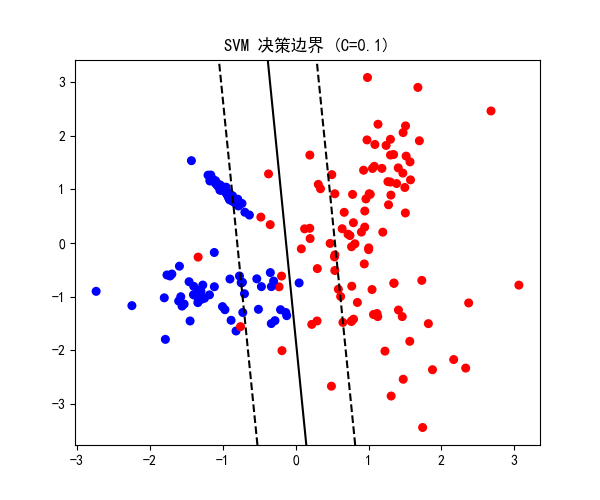
\includegraphics[width=\linewidth]{1.png}
        \caption{$C = 0.1$}
    \end{subfigure}
    \begin{subfigure}{0.3\textwidth}
        \centering
        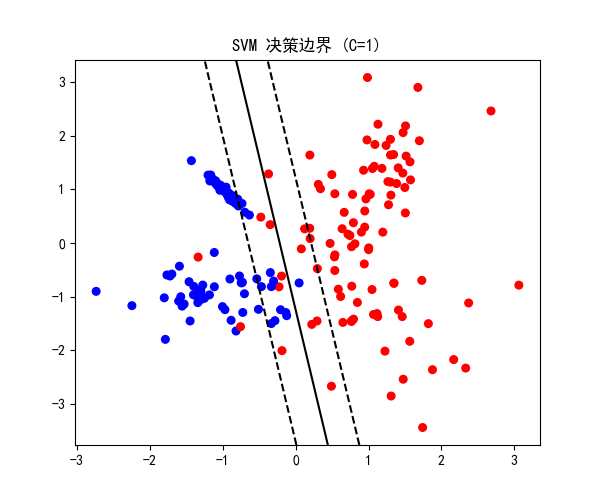
\includegraphics[width=\linewidth]{2.png}
        \caption{$C = 1$}
    \end{subfigure}
    \begin{subfigure}{0.3\textwidth}
        \centering
        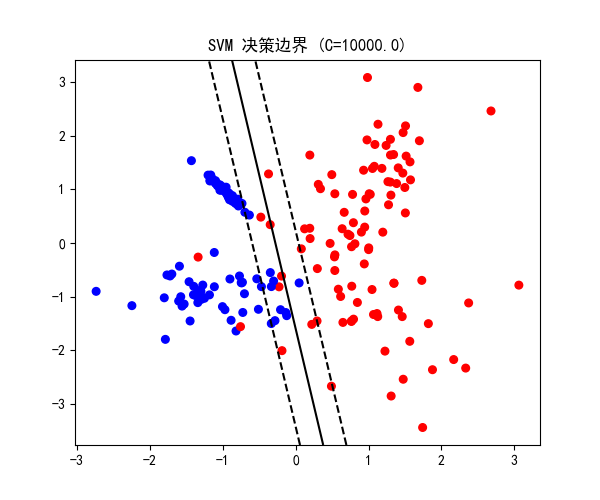
\includegraphics[width=\linewidth]{3.png}
        \caption{$C = 10^4$}
    \end{subfigure}
    \caption{不同 $C$ 值下的决策边界}
    \label{fig:svm_c}
\end{figure}

\begin{figure}
    
\end{figure}

\subsection{基于鸢尾花数据集的线性 SVM}
对鸢尾花数据集进行训练，仅选取 Setosa 与 Versicolor 进行二分类任务。绘制 PR 和 ROC 曲线并计算 F1 值。

\subsubsection{代码}
\begin{lstlisting}[language=python]
iris = load_iris()
X = iris.data
y = iris.target
X = X[y != 2]
y = y[y != 2]

X_train, X_test, y_train, y_test = train_test_split(
    X, y, test_size=0.3, random_state=42
)
scaler = StandardScaler()
X_train = scaler.fit_transform(X_train)
X_test = scaler.transform(X_test)
clf = SVC(kernel='linear', probability=True)
clf.fit(X_train, y_train)
\end{lstlisting}

\subsubsection{结果分析}
模型表现良好，PR 曲线完全贴合右上角，ROC 曲线完全贴合左上角，AUC 值接近 1。同时得到 $F1 = 1$，说明模型在精确率和召回率上平衡性较好。如图 \ref{fig:svm_iris_pr_roc} 所示。

\begin{figure}[htbp]
    \centering
    \begin{subfigure}{0.45\textwidth}
        \centering
        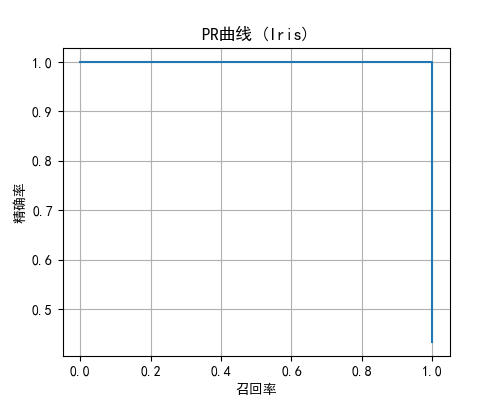
\includegraphics[width=\linewidth]{4.png}
        \caption{PR 曲线}
    \end{subfigure}
    \begin{subfigure}{0.45\textwidth}
        \centering
        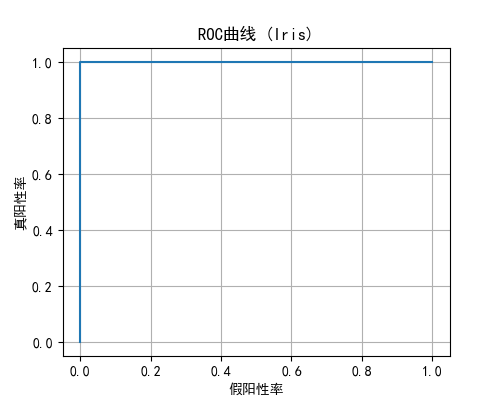
\includegraphics[width=\linewidth]{5.png}
        \caption{ROC 曲线}
    \end{subfigure}
    \caption{鸢尾花数据集的 PR 和 ROC 曲线}
    \label{fig:svm_iris_pr_roc}
\end{figure}

\subsection{基于 Moons 数据集的 SVM 核技巧}
通过使用 linear、poly、rbf 三种核函数，比较不同核函数在非线性数据集上的分类效果。

\subsubsection{代码}
\begin{lstlisting}[language=python]
X, y = make_moons(n_samples=500, noise=0.2, random_state=42)
X_train, X_test, y_train, y_test = train_test_split(
    X, y, test_size=0.3, random_state=42
)
scaler = StandardScaler()
X_train = scaler.fit_transform(X_train)
X_test = scaler.transform(X_test)
kernels = ["linear", "poly", "rbf"]
for k in kernels:
    clf = SVC(kernel=k, probability=True)
    clf.fit(X_train, y_train)
    y_score = clf.predict_proba(X_test)[:, 1]
    y_pred = clf.predict(X_test)
\end{lstlisting}

\subsubsection{实验结果}
图~\ref{fig:svm_moons_pr_roc} 展示了线性核的 PR 和 ROC 曲线，图~\ref{fig:svm_moons_pr_roc1} 展示了多项式核的 PR 和 ROC 曲线，图~\ref{fig:svm_moons_pr_roc2} 展示了 RBF 核的 PR 和 ROC 曲线。我们通过计算$F1$ 值来评估模型性能，得到：

\begin{itemize}
    \item 线性核：$F1 = 0.863013698630137$
    \item 多项式核：$F1 = 0.8794326241134752$
    \item RBF 核：$F1 = 0.9726027397260274$
\end{itemize}

\begin{figure}[htbp]
    \centering
    \begin{subfigure}{0.45\textwidth}
        \centering
        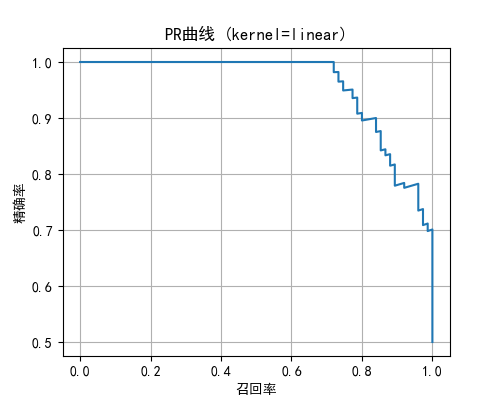
\includegraphics[width=\linewidth]{6.png}
        \caption{PR 曲线}
    \end{subfigure}
    \begin{subfigure}{0.45\textwidth}
        \centering
        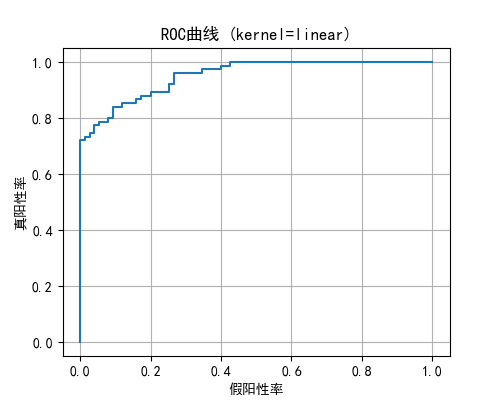
\includegraphics[width=\linewidth]{7.png}
        \caption{ROC 曲线}
    \end{subfigure}
    \caption{Moons 数据集的线性核 PR 和 ROC 曲线}
    \label{fig:svm_moons_pr_roc}
\end{figure}

\begin{figure}[htbp]
    \centering
    \begin{subfigure}{0.45\textwidth}
        \centering
        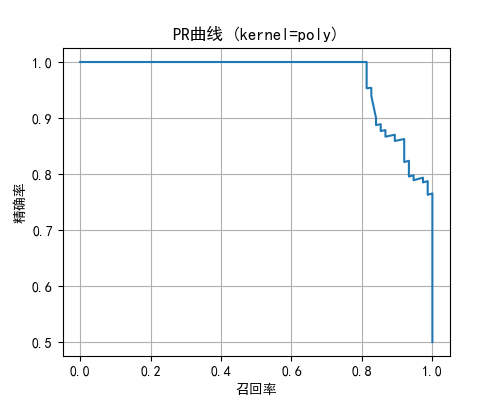
\includegraphics[width=\linewidth]{8.png}
        \caption{PR 曲线}
    \end{subfigure}
    \begin{subfigure}{0.45\textwidth}
        \centering
        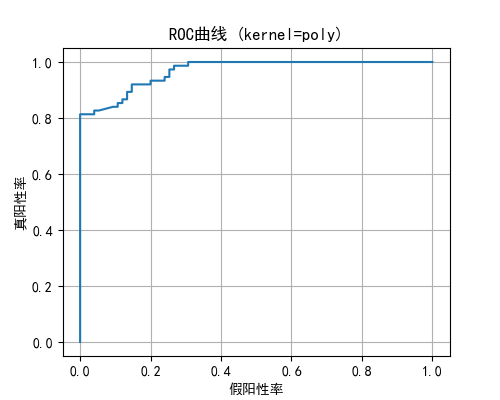
\includegraphics[width=\linewidth]{9.png}
        \caption{ROC 曲线}
    \end{subfigure}
    \caption{Moons 数据集的多项式核 PR 和 ROC 曲线}
    \label{fig:svm_moons_pr_roc1}
\end{figure}

\begin{figure}[htbp]
    \centering
    \begin{subfigure}{0.45\textwidth}
        \centering
        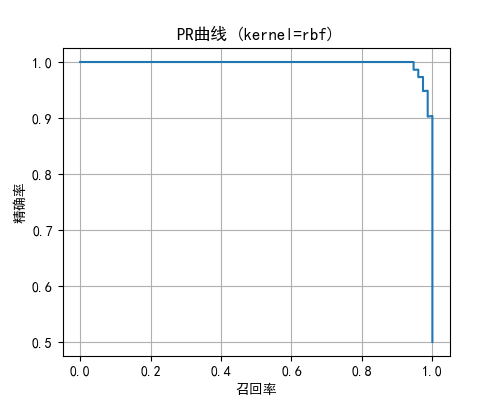
\includegraphics[width=\linewidth]{10.png}
        \caption{PR 曲线}
    \end{subfigure}
    \begin{subfigure}{0.45\textwidth}
        \centering
        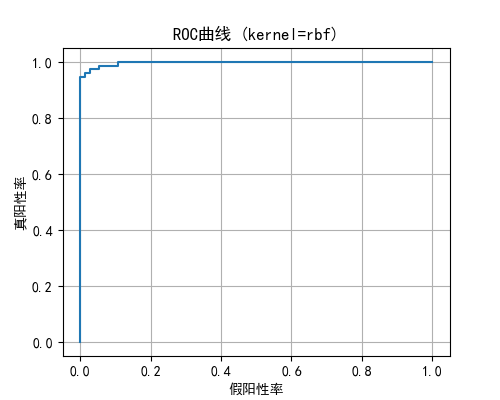
\includegraphics[width=\linewidth]{11.png}
        \caption{ROC 曲线}
    \end{subfigure}
    \caption{Moons 数据集的 RBF 核 PR 和 ROC 曲线}
    \label{fig:svm_moons_pr_roc2}
\end{figure}

不同核函数的 PR 和 ROC 曲线表现不同。RBF 核函数表现最佳，能够有效捕捉非线性结构；线性核效果较差；多项式核介于两者之间。

\section{总结}
通过本次实验，我理解了C 参数在 SVM 中的作用，掌握了不同核函数的使用方法。同时也明白了，支持向量机模型在小样本情形下具有良好的泛化能力，尤其在核技巧的辅助下能够处理复杂的非线性问题。

\newpage
\appendix
\section{完整代码}

\begin{lstlisting}[language=Python]
import numpy as np
import matplotlib.pyplot as plt
from sklearn.datasets import make_classification, load_iris, make_moons
from sklearn.model_selection import train_test_split
from sklearn.preprocessing import StandardScaler
from sklearn.svm import SVC
from sklearn.metrics import precision_recall_curve, roc_curve, f1_score, auc

plt.rcParams['font.sans-serif'] = ['SimHei']
plt.rcParams['axes.unicode_minus'] = False

def part1_svm_hard_soft():
    X, y = make_classification(
        n_samples=200,
        n_features=2,
        n_informative=2,
        n_redundant=0,
        random_state=25
    )

    for C in [0.1, 1, 1e4]:
        clf = SVC(kernel='linear', C=C)
        clf.fit(X, y)
        title = f"SVM 决策边界 (C={C})"
        plt.figure(figsize=(6, 5))
        plt.scatter(X[:, 0], X[:, 1], c=y, cmap='bwr', s=30)

        xlim = plt.xlim()
        ylim = plt.ylim()
        xx = np.linspace(xlim[0], xlim[1], 200)
        yy = np.linspace(ylim[0], ylim[1], 200)
        YY, XX = np.meshgrid(yy, xx)
        xy = np.vstack([XX.ravel(), YY.ravel()]).T

        Z = clf.decision_function(xy).reshape(XX.shape)
        plt.contour(XX, YY, Z, colors='k', levels=[-1, 0, 1], linestyles=['--', '-', '--'])
        plt.title(title)
        plt.show()

def part2_iris_svm():
    iris = load_iris()
    X = iris.data
    y = iris.target

    X = X[y != 2]
    y = y[y != 2]

    X_train, X_test, y_train, y_test = train_test_split(
        X, y, test_size=0.3, random_state=42
    )

    scaler = StandardScaler()
    X_train = scaler.fit_transform(X_train)
    X_test = scaler.transform(X_test)

    clf = SVC(kernel='linear', probability=True)
    clf.fit(X_train, y_train)

    y_score = clf.predict_proba(X_test)[:, 1]

    precision, recall, _ = precision_recall_curve(y_test, y_score)
    plt.figure(figsize=(5, 4))
    plt.plot(recall, precision)
    plt.title("PR曲线 (Iris)")
    plt.xlabel("召回率")
    plt.ylabel("精确率")
    plt.grid()
    plt.show()

    fpr, tpr, _ = roc_curve(y_test, y_score)
    plt.figure(figsize=(5, 4))
    plt.plot(fpr, tpr)
    plt.title("ROC曲线 (Iris)")
    plt.xlabel("假阳性率")
    plt.ylabel("真阳性率")
    plt.grid()
    plt.show()

    y_pred = clf.predict(X_test)
    print("Iris F1 Score:", f1_score(y_test, y_pred))

def part3_moons_svm():
    X, y = make_moons(n_samples=500, noise=0.2, random_state=42)

    X_train, X_test, y_train, y_test = train_test_split(
        X, y, test_size=0.3, random_state=42
    )

    scaler = StandardScaler()
    X_train = scaler.fit_transform(X_train)
    X_test = scaler.transform(X_test)

    kernels = ["linear", "poly", "rbf"]

    for k in kernels:
        clf = SVC(kernel=k, probability=True)
        clf.fit(X_train, y_train)

        y_score = clf.predict_proba(X_test)[:, 1]
        y_pred = clf.predict(X_test)

        precision, recall, _ = precision_recall_curve(y_test, y_score)
        plt.figure(figsize=(5, 4))
        plt.plot(recall, precision)
        plt.title(f"PR曲线 (kernel={k})")
        plt.xlabel("召回率")
        plt.ylabel("精确率")
        plt.grid()
        plt.show()

        fpr, tpr, _ = roc_curve(y_test, y_score)
        plt.figure(figsize=(5, 4))
        plt.plot(fpr, tpr)
        plt.title(f"ROC曲线 (kernel={k})")
        plt.xlabel("假阳性率")
        plt.ylabel("真阳性率")
        plt.grid()
        plt.show()

        print(f"F1 分数 (kernel={k}):", f1_score(y_test, y_pred))

if __name__ == "__main__":
    part1_svm_hard_soft()
    part2_iris_svm()
    part3_moons_svm()
\end{lstlisting}

\end{document}